\chapter{Linear Regression}


\section{Introduction}
Linear regression is the “work horse” of statistics and (supervised) machine learning. When augmented with kernels or other forms of basis function expansion, it can model also nonlinear relationships. And when the Gaussian output is replaced with a Bernoulli or multinoulli distribution, it can be used for classification, as we will see below. So it pays to study this model in detail.

In the simplest approach,we can directly construct an appropriate function $y(\vec{x})$ whose values for new inputs $\vec{x}$ constitute the predictions for the corresponding values of $t$.More generally,from a probabilistic perspective,we aim to model the predictive distribution $p(t|x)$ because this expresses the uncertainty about the value of $t$ for each value of $x$.

\section{Representation}
The simplest linear model for regression is \textbf{linear regression} that involves a linear combination of the input variables
\begin{equation}
y(\vec{x},\vec{w}) = w_0+w_1x_1+...+w_Dx_D
\end{equation}
where $\vec{x}=(x_1,...,x_D)^T$.

Linear regression can be made to model non-linear relationships by replacing $\vec{x}$ with some non-linear function of the inputs, $\phi(\vec{x})$.Consider the linear combinations of fixed nonlinear functions of the input variables,of the form
\begin{equation}
y(\vec{x},\vec{w}) = w_0+\sum_{j=1}^{M-1}w_j\phi_j(x) 
=\sum_{j=0}^{M-1}w_j\phi_j(x) = \vec{w}^T\phi(x)
\end{equation}
where $\phi_j(x)$ are known as \textbf{basis functions},
$\vec{w}=(w_0,...,w_{M-1})^T$ and $\phi=(\phi_0,...,\phi_{M-1})^T$.
This is known as \textbf{basis function expansion}. (Note that the model is still linear in the parameters $\vec{w}$, so it is still called linear regression; the importance of this will become clear below.) A simple example are polynomial basis functions, where the model has the form
\begin{equation}
\phi(x)=(1, x, \cdots, x^d)
\end{equation}


As before,we assume that the target variable is given by a deterministic function $y(\vec{x},\vec{w})$ with additive Gaussian noise so that
\begin{equation}
t=y(\vec{x},\vec{w})+\epsilon
\end{equation}
where $\epsilon$ is a zero mean Gaussian random variable with precision(inverse variance) $\beta$.Thus
\begin{equation}\label{eqn:linear regression representation}
p(t|\vec{x},\vec{w},\beta)=\mathcal{N}(t|h(\vec{x},\vec{w}),\beta^{-1})
\end{equation}
or 
\begin{eqnarray}
& y(\vec{x}) = \vec{w}^T\vec{x}+\epsilon \\
& p(y|\vec{x},\vec{\theta})=\mathcal{N}(y|\vec{w}^T\vec{x}, \sigma^2) \\
\end{eqnarray}
where $\vec{w}$ (\textbf{weight vector}) and $\vec{x}$ are extended vectors, $\vec{x}=(1,x)$, $\vec{w}=(b,w)$ and $\epsilon$ has a \textbf{Gaussian} or \textbf{normal} distribution.$w_0$ is the intercept or \textbf{text}

 
%\begin{eqnarray}
%& y(\vec{x}) = \vec{w}^T\phi(\vec{x})+\epsilon \\
%& p(y|\vec{x},\vec{\theta})=\mathcal{N}(y|\vec{w}^T\phi(\vec{x}), \sigma^2)
%\end{eqnarray}


\section{Maximum likelihood estimations(least squares)}
Assume the training examples are \textbf{independently and identically distributed(IID)},we obtain the \textbf{likelihood function},which is a function of adjustable parameters $\vec{w}$ and $\beta$,in the form
\begin{align}\label{eqn:linear regression likelihood}
p(\vec{t}|\vec{X},\vec{w},\beta) =
\prod_{n=1}^{N}\mathcal{N}(t_n|\vec{w}^T\phi(\vec{x_n}),\beta^{-1})
\end{align}
we can write the \textbf{log-likelihood} (logarithm of the likelihood) function as follows:
\begin{equation}
\ell(\vec{\theta}) \triangleq \log p(\mathcal{D}|\vec{\theta})
\end{equation}
A common way to estimate the parameters of a statistical model is to compute the MLE(Maximum likelihood estimations),which is defined as
\begin{equation}
\vec{\hat{\theta}}=\arg\max_\theta{\log p(\mathcal{D}|\vec{\theta})}
\end{equation}

Instead of maximizing the log-likelihood, we can equivalently minimize the \textbf{negative log likelihood} or \textbf{NLL}:
\begin{equation}
\text{NLL}(\vec{\theta}) \triangleq -\ell(\vec{\theta})=-\log p(\mathcal{D}|\vec{\theta})
\end{equation}

The NLL formulation is sometimes more convenient, since many optimization software packages are designed to find the minima of functions, rather than maxima.

Now let us apply the method of MLE to the linear regression setting. Inserting the definition of the Gaussian into the above, we find that the log likelihood is given by
\begin{align}
\ell(\vec{\theta}) &= \log p(\vec{T}|\vec{w},\beta) \\
&=\sum_{n=1}^{N}\log \mathcal{N}(t_n|\vec{w}^T\phi(\vec{x_n}),\beta^{-1}) \\
&=\sum\limits_{i=1}^N \log\left[\dfrac{1}{\sqrt{2\pi}\sigma}\exp\left(-\dfrac{1}{2\sigma^2}(y_i-\vec{w}^T\vec{x}_i)^2\right)\right] \\
&=\dfrac{N}{2}\log \beta-\dfrac{N}{2}\log (2\pi)-\beta E_D(\vec{w}) \\
&=-\dfrac{1}{2\sigma^2}\text{RSS}(\vec{w})-\dfrac{\vec{w}}{2}\log(2\pi\sigma^2)
\end{align}
where the sum-of-squares error function is defined by
\begin{equation}
E_D(\vec{w}) =
\dfrac{1}{2}\sum_{n=1}^{N}\{t_n-\vec{w}^T\phi(\vec{x_n}) \}^2
\end{equation}
RSS stands for \textbf{residual sum of squares} and is defined by
\begin{equation}
\text{RSS}(\vec{w}) \triangleq \sum\limits_{i=1}^N (t_i-\vec{w}^T\vec{x}_i)^2
\end{equation}
The RSS can also be written as the square of the $\ell_2$ \textbf{norm} of the vector of residual errors:
\begin{equation}
RSS(\vec{w}) = \parallel\epsilon\parallel_2^2 = \sum_{i=1}^{N}\epsilon_i^2
\end{equation}
where $\epsilon_i = (t_i - \vec{w}^T\vec{x_i})$.

There two ways to compute the optimal solution of likelihood function.

\subsection{Derivations of the MLE}
We see that maximizing the likelihood function under a conditional Gaussian noise distribution for a linear model is equivalent to $\vec{w}$ minimizing the RSS(or $E_D$), so this method is known as \textbf{least squares}.The gradient of the log likelihood function takes the form
\begin{equation}
\nabla\log p(\vec{t}|\vec{w},\beta)
=\sum_{n=1}^{N}\{t_n-\vec{w}^T\phi(\vec{x_n}) \}\phi(\vec{x_n})^T
\end{equation}

Let's drop constants with respect to $\vec{w}$ and NLL can be written as
\begin{equation}
\text{NLL}(\vec{w}) = \dfrac{1}{2}\sum\limits_{i=1}^N (y_i-\vec{w}^T\vec{\phi}_i)^2
\end{equation}

Define $\vec{y}=(t_1,t_2,\cdots,t_N)$, $\vec{\Phi}=\left(\begin{array}{c}\vec{\phi}_1^T \\ \vec{\phi}_2^T \\ \vdots \\ \vec{\phi}_N^T\end{array}\right)$, then we can rewritten the objective in a form that is more amendable to differentiation:
\begin{align}
\text{NLL}(\vec{w}) &= \dfrac{1}{2}(\vec{t}-\vec{\Phi}\vec{w})^T(\vec{t}-\vec{\Phi}\vec{w})\\
&= \dfrac{1}{2} [\vec{w^T} (\vec{\Phi}^T\vec{\Phi})\vec{w} - \vec{t}^T\vec{\Phi}\vec{w}- \vec{w}^T\vec{x}^T\vec{t}  +\vec{t}^T\vec{t}]			\\
\Rightarrow
\dfrac{\partial}{\partial \vec{w}}\text{NLL} &= \dfrac{1}{2} \vec{w^T} (\vec{\Phi}^T\vec{\Phi})\vec{w} -\vec{w}^T(\vec{\Phi}^T\vec{t}) 
\end{align}

where
$\begin{cases}
\vec{\Phi} = \begin{bmatrix}
&\vec{\Phi_1^T} \\
&\vec{\Phi_2^T} \\
& ... \\
&\vec{\Phi_n^T}
\end{bmatrix} \\	
\vec{\Phi^T}\vec{\Phi} =
\begin{bmatrix}
\vec{\Phi_1} & \vec{\Phi_2} & ...&\vec{\Phi_n}
\end{bmatrix} 
\cdot
\begin{bmatrix}
&\vec{\Phi_1^T} \\
&\vec{\Phi_2^T} \\
& ... \\
&\vec{\Phi_N^T}
\end{bmatrix}  = \sum\limits_{i=1}^{N}\vec{\phi_i}\vec{\phi_i^T} = \textbf{sum of squares matrix} \\
\end{cases}$

Note that $\vec{\Phi}$ is an $N\times M$ matrix,called the \textbf{design matrix},whose elements are given by $\Phi_{nj}=\phi_j(\vec{x_n})$ so that
\begin{equation}
\vec{\Phi}=
\begin{bmatrix}
\phi_0(\vec{x_1}) &	\phi_1(\vec{x_1}) &...&\phi_{M-1}(\vec{x_1}) \\
\phi_0(\vec{x_2}) & \phi_1(\vec{x_2}) &...&\phi_{M-1}(\vec{x_2}) \\
\vdots &\vdots &\vdots&\vdots \\
\phi_0(\vec{x_N})& \phi_1(\vec{x_{N}})& \cdot &\phi_{M-1}(\vec{x_N})\\
\end{bmatrix}
\end{equation}



When $\mathcal{D}$ is small(for example, $N < 1000$), we can use the following equation to compute $\vec{w}$ directly
\begin{equation}
\vec{w}_{ML}=\hat{\vec{w}}_{\mathrm{OLS}}=(\vec{\Phi}^T\vec{\Phi})^{-1}\vec{\Phi}^T\vec{t}
\end{equation}

The corresponding solution $\hat{\vec{w}}_{\mathrm{OLS}}$ to this linear system of equations is called the \textbf{ordinary least squares} or \textbf{OLS} or \textbf{normal equation} solution.

\begin{proof}
We now state without proof some facts of matrix derivatives (we won’t need all of these at this section).
\begin{eqnarray}
trA &\triangleq& \sum\limits_{i=1}^n A_{ii} \nonumber \\
\frac{\partial}{\partial A}AB &=& B^T \\
\frac{\partial}{\partial A^T}f(A) &=& \left[\frac{\partial}{\partial A}f(A)\right]^T \label{eqn:matrix-1} \\
\frac{\partial}{\partial A}ABA^TC &=& CAB+C^TAB^T \label{eqn:matrix-2} \\
\frac{\partial}{\partial A}|A| &=& |A|(A^{-1})^T
\end{eqnarray}

Then,
\begin{eqnarray*}
\text{NLL}(\vec{w}) &=& \frac{1}{2N}(\vec{X}\vec{w}-\vec{y})^T(\vec{X}\vec{w}-\vec{y}) \\
\frac{\partial \text{NLL}}{\partial\vec{w}} 
&=& \frac{1}{2} \frac{\partial}{\partial\vec{w}} (\vec{w}^T\vec{X}^T\vec{X}\vec{w}-\vec{w}^T\vec{X}^T\vec{y}-\vec{y}^T\vec{X}\vec{w}+\vec{y}^T\vec{y}) \\
&=& \frac{1}{2} \frac{\partial}{\partial\vec{w}} (\vec{w}^T\vec{X}^T\vec{X}\vec{w}-\vec{w}^T\vec{X}^T\vec{y}-\vec{y}^T\vec{X}\vec{w}) \\
&=& \frac{1}{2} \frac{\partial}{\partial\vec{w}}  \\
&=& \frac{1}{2} \frac{\partial}{\partial\vec{w}} (tr\vec{w}^T\vec{X}^T\vec{X}\vec{w}-2tr\vec{y}^T\vec{X}\vec{w})
\end{eqnarray*}

Combining Equations \ref{eqn:matrix-1} and \ref{eqn:matrix-2}, we find that 
\begin{equation*}
\frac{\partial}{\partial A^T}ABA^TC = B^TA^TC^T+BA^TC
\end{equation*}

Let $A^T=\vec{w}, B=B^T=\vec{X}^T\vec{X}$, and $C=I$, Hence,
\begin{eqnarray}
\frac{\partial \text{NLL}}{\partial\vec{w}} &=& \frac{1}{2} (\vec{X}^T\vec{X}\vec{w}+\vec{X}^T\vec{X}\vec{w} -2\vec{X}^T\vec{y}) \nonumber \\
						   &=& \frac{1}{2} (\vec{X}^T\vec{X}\vec{w} - \vec{X}^T\vec{y}) \nonumber \\
\frac{\partial \text{NLL}}{\partial\vec{w}} &=& 0 \Rightarrow \vec{X}^T\vec{X}\vec{w} - \vec{X}^T\vec{y} =0 \nonumber \\
\vec{X}^T\vec{X}\vec{w} &=& \vec{X}^T\vec{y} \label{eqn:normal-equation} \\
\hat{\vec{w}}_{\mathrm{OLS}} &=& (\vec{X}^T\vec{X})^{-1}\vec{X}^T\vec{y} \nonumber
\end{eqnarray}
\end{proof}
Equation \ref{eqn:normal-equation} is known as the \textbf{normal equation}.
\begin{proof}
Consider $\mathbf{vector-vector}$ differentiation,if $\mathbf{A}$ is not a function of $\vec{x}$ then
\begin{equation}
\dfrac{\partial\vec{X}^TA\vec{X}}{\partial\vec{X}} = \vec{X}^T(\mathbf{A}+\mathbf{A}^T) = (\mathbf{A}+\mathbf{A}^T)\vec{X}
\end{equation}
\end{proof}
Then,we can derivate $\dfrac{\partial NLL}{\partial \vec{w}}$
\begin{eqnarray}
g(\vec{w}) &= \dfrac{\partial NLL}{\partial\vec{w}} \\
&=\vec{\Phi}^T\vec{\Phi}\vec{w} - \vec{\Phi}^T\vec{y}			
\end{eqnarray}
Setting the derivative to zero,we get
\begin{equation}
	\vec{w} = (\vec{X}^T\vec{X})^{-1}\vec{x}^T\vec{y}
\end{equation}

\subsection{Geometric interpretation}

See Figure \ref{fig:graphical-interpretation-of-OLS}.
\begin{figure}[hbtp]
\centering
    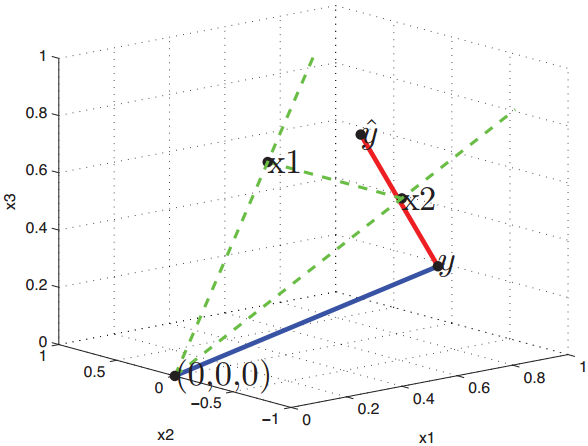
\includegraphics[scale=.50]{graphical-interpretation-of-OLS.png}
\caption{Graphical interpretation of least squares for $N=3$ examples and $D=2$ features. $\tilde{\vec{x}}_1$ and $\tilde{\vec{x}}_2$˜ are vectors in $\mathbb{R}^3$; together they define a 2D plane. $\vec{y}$ is also a vector in $\mathbb{R}^3$ but does not lie on this 2D plane. The orthogonal projection of $\vec{y}$ onto this plane is denoted $\hat{\vec{y}}$. The red line from $\vec{y}$ to $\hat{\vec{y}}$ is the residual, whose norm we want to minimize. For visual clarity, all vectors have been converted to unit norm.}
\label{fig:graphical-interpretation-of-OLS} 
\end{figure}
Given that
\begin{eqnarray}
\vec{X} = \begin{bmatrix}
\vec{x_1}^T &\\
\vec{x_2}^T &\\
 ...        &\\
\vec{x_N}^T
\end{bmatrix} 
= \begin{bmatrix}
\vec{\tilde{x_1}} & \vec{\tilde{x_1}} & ... &\vec{\tilde{x_D}}
\end{bmatrix}\\
\vec{y} = \begin{bmatrix}
y_1 \\
y_2 \\
... \\
y_n
\end{bmatrix} 
\end{eqnarray}
We seek a vector $\hat{\vec{y}} \in \mathbb{R}^N$ that lies in the column linear space of $\vec{X}$ and is as close as possible to $\vec{y}$,i.e.,we want to find
\begin{eqnarray}
\hat{\vec{y}} \in span(\vec{X}) \\
\Rightarrow \hat{\vec{y}} = \vec{X}\vec{w} = w_1\vec{\tilde{x_1}}+\cdot\cdot\cdot+w_D\vec{\tilde{x_D}} \\
\vec{\hat{y}}=\arg\min\limits_{\hat{\vec{y}} \in \text{span} (\{\vec{\tilde{x_1}},...,\vec{\tilde{x_D}}\})}
\end{eqnarray}

To minimize the norm of the residual, $\vec{y}-\hat{\vec{y}}$, we want the residual vector to be orthogonal to every column of $\vec{X}$,so˜ $\tilde{\vec{x}}_j(\vec{y}-\hat{\vec{y}})=0$ for $j=1:D$. Hence
\begin{equation}\begin{split}
\tilde{\vec{x}}_j(\vec{y}-\hat{\vec{y}})=0 & \Rightarrow \vec{X}^T(\vec{y}-\vec{X}\vec{w})=0 \\
                                           & \Rightarrow \vec{w}=(\vec{X}^T\vec{X})^{-1}\vec{X}^T\vec{y}
\end{split}\end{equation}


\subsection{Sequential learning}
Batch techniques,such as the maximum likelihood solution,which involves processing the entire training set in one go(pass),can be computationally costly for large data sets.If the data set is sufficiently large,it may be worthwhile to use \textbf{sequential} algorithms,known as \textbf{on-line} algorithms.
When $\mathcal{D}$ is large, use \textbf{stochastic gradient descent(SGD)},also known as sequential gradient descent.
\begin{align}
E &=\sum_{n}E_n \\
\vec{w}^{\tau+1} &= \vec{w}^{\tau}-\eta\nabla E_n
\end{align}
where $\tau$ denotes the iteration number,the $\eta$ is a learning rate parameter.For the case of sum-of-squares error function,this gives
\begin{equation}
\vec{w}^{\tau+1} = \vec{w}^{\tau}-\eta(t_n-\vec{w}^{(\tau)T}\phi_n)\phi_n
\end{equation}
where $\phi_n=\phi(\vec{x_n})$.This is known as the \textbf{least-mean-squares} or the LMS algorithm.


\begin{align}
\because \dfrac{\partial}{\partial w_i}\text{NLL}(\vec{w})=& \sum\limits_{i=1}^N (\vec{w}^T\vec{x}_i-y_i)x_{ij} \\
\therefore w_j=& w_j - \alpha\dfrac{\partial}{\partial w_j}\text{NLL}(\vec{w}) \nonumber \\
                  =& w_j - \sum\limits_{i=1}^N \alpha(\vec{w}^T\vec{x}_i-y_i)x_{ij} \\
\therefore \vec{w}=& \vec{w}-\alpha(\vec{w}^T\vec{x}_i-y_i)\vec{x}
\end{align}


\section{Ridge regression(MAP)}
One problem with ML estimation is that it can result in over-fitting. In this section, we discuss a way to ameliorate this problem by using MAP estimation with a Gaussian prior.

\subsection{Basic idea}
We can encourage the parameters to be small, thus resulting in a smoother curve, by using a zero-mean Gaussian prior:
\begin{equation}
p(\vec{w})=\prod\limits_j \mathcal{N}(w_j|0,\tau^2)
\end{equation}
where $1/\tau^2$ controls the strength of the prior. The corresponding MAP estimation problem becomes
\begin{equation}
\arg\max_{\vec{w}} \sum\limits_{i=1}^N \log{\mathcal{N}(t_i|w_0+\vec{w}^T\vec{\phi}_i,\sigma^2)}+\sum\limits_{j=1}^D \log{\mathcal{N}(w_j|0,\tau^2)}
\end{equation}

It is a simple exercise to show that this is equivalent to minimizing the following
\begin{align}\label{eqn:Ridge-regression-J}
J(\vec{w})&=E_D(\vec{w})+\lambda E_W(\vec{w}) \\
&=\dfrac{1}{N}\sum\limits_{i=1}^N (y_i-(w_0+\vec{w}^T\vec{x}_i))^2+\lambda\lVert\vec{w}\rVert^2 , \lambda \triangleq \dfrac{\sigma^2}{\tau^2}
\end{align}
where the first term is the MSE/ NLL as usual, and the second term, $\lambda \geq 0$, is the regularization coefficient that controls the complexity penalty.
Here $E_W(\vec{w})$ is one of the simplest forms of regularizer given by the sum-of-squares of the weight vector elements.
\begin{equation}
E_W(\vec{w})=\dfrac{1}{2}\vec{w}^T\vec{w}
\end{equation}
This particular choice of regularizer is known as \textbf{weight decay}.

The corresponding solution is given by
\begin{equation}\label{eqn:Ridge-regression-solution}
\hat{\vec{w}}_{\mathrm{ridge}}=(\lambda\vec{I}_D+\vec{\Phi}^T\vec{\Phi})^{-1}\vec{\Phi}^T\vec{t}
\end{equation}

This technique is known as \textbf{ridge regression},or \textbf{penalized least squares}. In general, adding a Gaussian prior to the parameters of a model to encourage them to be small is called $\ell_2$ \textbf{regularization} or \textbf{weight decay}. Note that the offset term $w_0$ is not regularized, since this just affects the height of the function, not its complexity.

We will consider a variety of different priors in this book. Each of these corresponds to a different form of \textbf{regularization}. This technique is very widely used to prevent overfitting.

\subsection{Multiple outputs}
Now consider the case where we wish to predict $K>1$ target variables,which we denote collectively by the target vector $\vec{t}$.To use the same set of basis functions to model all the components of the target vector so that
\begin{equation}
\vec{y}(\vec{x},\vec{w}) = \vec{W}^T\phi(x)
\end{equation}
where $\vec{y}$ is a $K$-dimensional column vector,$\vec{W}$ is an $M\times K$ matrix of parameters.

The conditional distribution of the target vector is an isotropic Gaussian
\begin{equation}
p(\vec{t}|\vec{x},\vec{W},\beta) =
\mathcal{N}(\vec{t}|\vec{W}^T\phi(x,\beta^{-1}\vec{I}))
\end{equation}

The log likelihood function is then given by 
\begin{align}
\ln p(\vec{T}|\vec{X},\vec{W},\beta) 
&=\sum_{n=1}^{N}\ln \mathcal{N}(\vec{t_n}|\vec{W}^T\phi(x_n),\beta^{-1}\vec{I}) \\
&=\dfrac{NK}{2}\ln(\dfrac{\beta}{2\pi}) 
 -\dfrac{\beta}{2}\sum_{n=1}^{N}\parallel \vec{t_n}-\vec{W}^T\phi(x_n)\parallel^2
\end{align}
We maximize this function with respect to $\vec{W}$,giving
\begin{equation}
\vec{W}_{ML} = (\vec{\Phi}^T\vec{\Phi})^{-1}\vec{\Phi}^T\vec{T}
\end{equation}


\subsection{Numerically stable computation *}

\begin{equation}\label{eqn:Ridge-regression-SVD}
\hat{\vec{w}}_{\mathrm{ridge}}=\vec{V}(\vec{Z}^T\vec{Z}+\lambda\vec{I}_N)^{-1}\vec{Z}^T\vec{y}
\end{equation}


\subsection{Connection with PCA *}


\subsection{Regularization effects of big data}
Regularization is the most common way to avoid overfitting. However, another effective approach — which is not always available — is to use lots of data. It should be intuitively obvious that the more training data we have, the better we will be able to learn.

In domains with lots of data, simple methods can work surprisingly well (Halevy et al. 2009). However, there are still reasons to study more sophisticated learning methods, because there will always be problems for which we have little data. For example, even in such a data-rich domain as web search, as soon as we want to start personalizing the results, the amount of data available for any given user starts to look small again (relative to the complexity of the problem).

\section{The Bias-Variance Decomposition}
\subsubsection{representation}
Data representation:
N observations of x,wiritten 
$X \equiv (x_1,x_2,...,x_n)^T$
together with corresponding observations of the values of t,denoted 
$t \equiv (t_1,t_2,...t_N)^T$.
\begin{equation}
t_i = f(\vec{x_i}) + \epsilon 
\end{equation}
where the noise $ \epsilon $ has zero mean and variance $ \sigma^2 $.
Find a function \[ \hat{f}(x) \] that approximates the true function \[ t = f(\vec{x}) \] as well as possible.Make "as well as possible" precise  by measuring the mean squared error between y and $ \hat{f}(x) $,we want $ (t - \hat{f}(x))^2 $ to be minimal.
Hypothesis function(model representation):
$y(x,\bold w)= w_0+w_1x+w_2x^2+...+w_Mx^M = \sum_{j=0}^{M}w_jx^j$
M is the order of the polynomial,and $x^j$ denotes $x$ raised to the power of $j$.The polynomial coefficients $w_0,...w_M$ are
collectively denoted by the vector $\mathbf{w}$.

Error Function(Sum of squares of errors between predictions $y(x_n,w)$ for each data point $x_n$ and the corresponding target values $t_n$,so that we minimize:
\begin{equation}
E(\bold w)=\frac{1}{2}\sum_{n=1}^{N}\{y(x_n,\bold w)-t_n \}^2
\end{equation}
root-mean-squre(RMS) error defined by
\begin{equation} 
E_{RMS} = \sqrt[2]{2E(\bold w^*)/N}
\end{equation}
Penalized(regularized) error function
\begin{equation}
\widetilde{E}(\textbf{w}) = \frac{1}{2}\sum_{n=1}^{N}\{y(x_n,\textbf{w}-t_n\}^2 + \frac{1}{2} \parallel \textbf{w} \parallel^2
\end{equation}
where $\parallel \textbf{w} \parallel^2 \equiv \textbf{w}^T\textbf{w}=w_0^2+w_1^2+...+w_M^2$

\subsubsection{Loss function for regression}
\begin{equation}
\mathbb{E}[\mathit{L}] = \iint\mathit{L}(t,y(\textbf{x}))p(\textbf{x},t)d\textbf{x}dt
\end{equation}
A common choice of loss function in squared loss given by 
\begin{eqnarray}
\mathit{L}(t,y(\textbf{x})) = \{y(\textbf{x}) - t\}^2 \\
\mathbb{E}[\mathit{L}] = \iint\{y(\textbf{x}) - t\}^2 p(\textbf{x},t)d\textbf{x}dt.
\end{eqnarray}
Minimize $ \mathbb{E}[\mathit{L}] $ by using the calculus of variations to give 
\begin{equation}
\frac{\delta\mathbb{E}[\mathit{L}]}{\delta y(\mathbf{x}))} = 2 \int\{ y(\mathbf{x} -t) \}p(\mathbf{x},t)dt = 0
\end{equation}
Solving for $ y(\textbf{x}) $ and using the sum and product rules of probability,we obtain
\begin{equation}
y(\textbf{x}) = \frac{\int tp(\textbf{x},t)dt}{p(\textbf{x})} = \int tp(t|\textbf{x})dt = \mathbb{E}[t|\textbf{x}]
\end{equation}

Let's derive this result in a slightly different way.Armed with knowledge that the optimal solution is the 
conditional expectation,we can expand the square term as follows
\begin{equation}
\{y(\textbf{x} -t)\}^2
= \{y(\textbf{x}) - \mathbb{E}[t|\textbf{x}] + \mathbb{E}[t|\textbf{x}] - t )\}^2 
= \{ y(\textbf{x}) - \mathbb{E}[t|\textbf{x}] \}^2 + 2\{ y(\textbf{x}) - \mathbb{E}[t|\textbf{x}] \}\{ \mathbb{E}[t|\textbf{x}]-t \} + \{ \mathbb{E}[t|\textbf{x}] -t \}^2
\end{equation}
where,$ \mathbb{E}[t|\textbf{x}] $ denote $ \mathbb{E}_{t}[t|\textbf{x}] $.Substitute into the loss function and perform the integral over t,we see the cross-term vanishes
\begin{align}\label{eqn:squared loss function}
\mathbb{E}[\mathit{L}]                                                           
&= \iint\{y(\textbf{x}) - t\}^2 p(\textbf{x},t)d\textbf{x}dt                    \\
&= \int \{ y(\textbf{x}) -\mathbb{E}[t|\textbf{x}] \}^2 p(\textbf{x})d\textbf{x} + 
\int\{ \mathbb{E}[t|\textbf{x}] - t \}^2 p(\textbf{x})d\textbf{x}               \\
&= \int \{ y(\textbf{x}) -h(\textbf{x}) \}^2 p(\textbf{x})d\textbf{x} +            
\int\{ h(\textbf{x}) - t \}^2 p(\textbf{x})d\textbf{x}                          \\
&= \int \{ y(\textbf{x}) -h(\textbf{x}) \}^2 p(\textbf{x})d\textbf{x} +            
\int\{ h(\textbf{x}) - t \}^2 p(\textbf{x},t)d\textbf{x}dt                      \\
\end{align}

\subsubsection{Decomposition}
For a popular choice,we use squared loss function,for which the optimal prediction is given by the conditional
expectation,which we denote by h(\textbf{x}) and which is given by 
\begin{equation}
h(\textbf{x}) = \mathbb{E}[t|\textbf{x}] = \int tp(t|\textbf{x})dt
\end{equation}

Consider the integrand of the first term of \ref{eqn:squared loss function},which for particular data set D takes the form
\begin{equation}
\{ y(\textbf{x};D) - h(\textbf{x}) \} ^2
\end{equation}
This quantity will be dependent on the particular data set D,so we take its average over the ensemble of data sets.
If we add and subtract the quantity $ \mathbb{E_D}[y(\textbf{x};D)] $ inside the braces,and then expand,we obtain
\begin{align}
\{ y(\textbf{x};D) - h(\textbf{x}) \} ^2 \\
=&\{y(\textbf{x};D) - \mathbb{E_D}[y(\textbf{x};D)] 
	+ \mathbb{E_D}[y(\textbf{x};D)] -h(\textbf{x})  \}^2         \\
=& \{ y(\textbf{x};D) -\mathbb{E}[y(\textbf{x};D)]    \}^2 
	+ \{ \mathbb{E_D}[y(\textbf{x};D)] - h(\textbf{x})\}^2
	+ 2\{ y(\textbf{x};D) - \mathbb{E_D}[y(\textbf{x};D)]\}\{ \mathbb{E_D}[y(\textbf{x};D)] -h(\textbf{x})\} \\
=& \underbrace{\{ y(\textbf{x};D) -\mathbb{E}[y(\textbf{x};D)]    \}^2} 
	+ \underbrace{\{ \mathbb{E_D}[y(\textbf{x};D)] - h(\textbf{x})\}^2}   \\
=&                    \color{red}{variance}                 +   \color{blue}{(bias)^2}  + (irreducible error)
\end{align}
The decomposition of the expected squared loss
\begin{equation}
\text{expected loss} = (bias)^2 + variance + noise
\end{equation}
where
\begin{eqnarray}
(bias)^2 = ... \\
variance = ... \\
noise = ...
\end{eqnarray}

The function $ y(\textbf{x}) $ we seek to determine enters only the first term,which will be minimized when $ y(\textbf{x}) $ is equal to $ \mathbb{E}[t|\textbf{x}] $,in which case this term will vanish.The second term is the variance of distribution of t,averaged over $ \textbf{x} $,representing the intrinsic variabilility of the target data and can be regarded as noise.It's the irreducible minimum value of the loss function.

More sophisticated loss function,Minkowski loss
\begin{equation}
\mathbb{E}[\mathit{L_q}] = \iint| y(\textbf{x}) - t |^q p(\textbf{x},t)d\textbf{x}dt
\end{equation}


\section{Bayesian linear regression}
Hold-out data can be used to determine model complexity but it will be 
computationally expensive and wasteful of valuable data.We therefore turn to a Bayesian treatment of linear regression,which will avoid the over-fitting problem of maximum likelihood,and which will also lead to automatic methods of determining model complexity using the training data.

\subsection{Parameter distribution}
First introduce a prior probability distribution over the model parameters.The likelihood function $p(\vec{t}|\vec{w})$ defined by \ref{eqn:linear regression likelihood} is the exponential of a quadratic function of $\vec{w}$,so the corresponding conjugate prior is
Gaussian
\begin{equation}
p(\vec{w}) = \mathcal{N}(\vec{w}|\vec{m_0},\vec{S}_0)
\end{equation}

The posterior distribution is proportional to the product of the likelihood and the prior.And the posterior will also be Gaussian due to the choice of conjugate Gaussian prior,which is derived in \ref{sec:Gaussian distribution}.
\begin{equation}\label{eqn:Bayes linear regression posterior}
p(\vec{w}|\vec{t}) = \mathcal{N}(\vec{w}|\vec{m}_N,\vec{S}_N)
\end{equation}
where 
\begin{align}
\vec{m}_N &=\vec{S}_N(\vec{S}_0^{-1}\vec{m}_0+\beta\vec{\Phi}^T\vec{t})\\
\vec{S}_N^{-1} &= \vec{S}_0^{-1}+\beta\vec{\Phi}^T\vec{\Phi}
\end{align}
Thus the maximum posterior weigh vector is simply given by $\vec{w}_{MAP}=\vec{m}_{N}$.If $N=0$ then the posterior distribution reverts to the prior.Furthermore,if data points arrive sequentially,then the posterior distribution at any stage acts as the prior distribution,such that the new posterior is again given.

A zero-mean isotropic Gaussian governed by a single precision parameter $\alpha$ so that
\begin{equation}
p(\vec{w}|\alpha) = \mathcal{N}(\vec{w}|\vec{0},\alpha^{-1}\vec{I})
\end{equation}
for which the posterior is given by
\begin{align}
\vec{m}_N &=\beta\vec{S}_N\vec{\Phi}^T\vec{t} \\
\vec{S}_N^{-1}&=\alpha\vec{I}+\beta\vec{\Phi}^T\vec{\Phi}
\end{align}

The log of posterior distribution is given by the sum of the log likelihood and the log of prior and,as a function of $\vec{w}$,takes the form
\begin{equation}
\log p(\vec{w}|\vec{t}) = 
-\dfrac{\beta}{2}\sum_{n=1}^{N}\{t_n-\vec{w}^T\phi(\vec{x}_n) \}^2-\dfrac{\alpha}{2}\vec{w}^T\vec{w}+const
\end{equation}
Maximization of this posterior w.r.t $\vec{w}$ is equivalent to minimization of the sum-of-squares error function with the addition of a quadratic regularization term,corresponding with $\lambda=\alpha/\beta$.



\subsection{Predictive distribution}
Evaluate the \textbf{predictive distribution} defined by
\begin{equation}
p(t|\vec{t},\alpha,\beta) = \int p(t|\vec{w},\beta)p(\vec{w}|\vec{t},\alpha,\beta)d\vec{w}
\end{equation}
The conditional distribution $p(t|\vec{x},\vec{w},\beta)$ of the target variable is given by \ref{eqn:linear regression representation},and the posterior weight distribution is given by \ref{eqn:Bayes linear regression posterior}.This involves the \textbf{convolution} of two Gaussian distributions.The predictive distribution take the form
\begin{equation}
p(t|x,\vec{t},\alpha,\beta) = \mathcal{N}(t|\vec{m}_N^T\phi(x),\sigma_N^2(\vec{x})
\end{equation}
where the variance $\sigma_N^2(\vec{x})$ is given by
\begin{equation}
\sigma_N^2(\vec{x})=\dfrac{1}{\beta}+\phi(\vec{x})^T\vec{S}_N\phi(\vec{x})
\end{equation}
The first term represents the noise on the data whereas the second term reflects the uncertainty associated with the parameters $\vec{w}$.










